% game24 - Solves a game 24 scenario
% Copyright (C) 2020 Tim Gesthuizen <tim.gesthuizen@yahoo.de>
%
% This program is free software: you can redistribute it and/or modify
% it under the terms of the GNU General Public License as published by
% the Free Software Foundation, either version 3 of the License, or
% (at your option) any later version.
%
% This program is distributed in the hope that it will be useful,
% but WITHOUT ANY WARRANTY; without even the implied warranty of
% MERCHANTABILITY or FITNESS FOR A PARTICULAR PURPOSE.  See the
% GNU General Public License for more details.
%
% You should have received a copy of the GNU General Public License
% along with this program.  If not, see <https://www.gnu.org/licenses/>.

\documentclass[11pt,a4paper]{article}
\author{Tim Gesthuizen}
\title{Game 24}
\usepackage{tikz}
\usetikzlibrary{trees,fit,arrows,positioning,shapes.geometric}
\usepackage{listings}
\usepackage[a4paper,bindingoffset=0.2in,%
  left=1in,right=1in,top=1in,bottom=1in,%
  footskip=.4in]{geometry}
\usepackage{mathptmx}
\setlength\parindent{0px}
\usepackage{hyperref}
\usepackage{xcolor}
\hypersetup{
    colorlinks,
    linkcolor={red!50!black},
    citecolor={blue!50!black},
    urlcolor={blue!80!black}
}
\usepackage{listings}
\lstdefinelanguage{scheme}
{
  morekeywords={car, cdr, cons, lambda, define, if, when, let},
  morecomment=[l]{;;},
  morestring=[b]",
  frame = single,
  keepspaces = true,
}
\lstalias{shell}{sh}
\definecolor{comment-green}{rgb}{0,0.6,0}
\definecolor{linenumber-gray}{rgb}{0.5,0.5,0.5}
\definecolor{string-mauve}{rgb}{0.58,0,0.82}
\lstset{
  backgroundcolor=\color{white},
  basicstyle=\footnotesize,
  breakatwhitespace=false,
  breaklines=true,
  captionpos=b,
  escapeinside={\%*}{*)},
  extendedchars=true,
  frame=single,
  keepspaces=true,
  numbers=left,
  numbersep=5pt,
  rulecolor=\color{black},
  showspaces=false,
  showstringspaces=true,
  showtabs=false,
  stepnumber=5,
  tabsize=4,
  title=\lstname
}
% colors
\lstset{
  commentstyle=\color{comment-green},
  keywordstyle=\color{blue},
  numberstyle=\tiny\color{linenumber-gray},
  stringstyle=\color{string-mauve}
}
\newcommand{\code}[1]{\textit{#1}}

\begin{document}

\maketitle

\tableofcontents

\section{Problem description}

A program shall be written that solves the \textit{Game of 24}.
In this game you are given 4 numbers and need to come up with a
selection of the 4 arithmetic operators $+$, $-$, $\cdot$ and $\div$ to
reduce these numbers to the number 24.
The numbers can be rearranged in any order and the order of the
operations can also be manipulated.
See figure~\ref{fig:trees} for examples of syntax trees.

\input{tikz/syntax-trees.inc}
\input{tikz/syntax-tree-construction.inc}

\section{Problem analysis}
\label{sec:analysis}

The problem is to construct all possible syntax trees and evaluate
them systematically.
Selecting the operators is not difficult:
We have a set $Operators = \{+, -, \cdot, \div\}$ and generate all
permutations of a multi-set $M$ such that $\vert M \vert = 3$.
\newcommand{\complexop}{{\vert Operators \vert}^3}
\newcommand{\opconnect}{4 \cdot 3 \cdot 3 \cdot 2 \cdot 2 \cdot 1}
This results in $\complexop$ combinations of
operators.

To create a syntax tree from the four operands and the three operators
we use the following algorithm:
Move the seven nodes of the tree into an array, where the four
numbers are placed in front of the three operators.
Now construct an arena from which the operator inputs can be
choosen. The initial bounds of the arena are $[0, 4)$.
The first operator two ``wire up'' will be array entry 4, at the end
of the arena.
Now repeat the following steps for all operators:
\begin{enumerate}
  \item Connect the left hand side of the operator with one of the
    elements in the arena. Swap the selected element to the last
    element in the arena and shrink the end of it by one.
  \item Connect the right hand side of the operator with one of the
    elements in the arena. Swap the operator with the selected
    operand. This is done as the operator is now fully connected and
    can be used as an input for the following operators.
\end{enumerate}
If the algorithm is executed as described here, at the end the first
element of the array will always be the root node of the tree. In the
implementation the last swap is omitted so that the root node of the
tree is always the last node.
In the implementation the operators use indices into the array to
refer to their left and right hand side operands. This means that
swapping the actual elements of the array will break the referencing
of the operator nodes.
Therefore an extra indirection is used where the indices of the real
nodes are stored in an array of indicis and only the indices in the
array are swapped.
Through this indirection it is possibly to virtually swap elements in
the array without changing the physical arrangement of the nodes in
memory.
Find an example of this algorithm in figure~\ref{fig:treecon}.

Given this algorithm the total number of different syntax tree
``forms'' is $\opconnect$.
There are $\complexop \cdot \opconnect = 11664$ different syntax trees
that need to be checked as a consequence.

\section{Design of the first iteration of the program}

The user enters the four numbers the program shall find solutions
for. The program then calculates all permutations and builds up the
syntax trees for them. If a syntax tree evaluates to 24, it is
printed.
It should be noted that all of this can be done in $\mathcal{O}(1)$
space.
The above requirements result in the following software parts:
\begin{enumerate}
\item {\tt main} and user interactions
\item Syntax tree creation and permutation
\item Syntax tree evaluation
\item Syntax tree printing
\end{enumerate}

\section{Code of the first iteration of the program}

\lstinputlisting[language=C]{iteration1.c}

\section{Problems with the first iteration}

The first iteration of the program does very well. On Tim Gesthuizens
laptop the program takes a little bit longer than a tenth of a second
to run.
Surprisingly, as shows in figure \ref{fig:opt-info-it1}, GCC is able to
fold most of the code into the \code{main} function.
Even the indirect call of \textit{iterateAllSyntaxTrees} to
\code{checkAndPrintCallback} is detected and inlined.
As shown in figure \ref{fig:perfit1}, the hottest part of the program
is the evaluation of syntax trees.
As expected the compiler was not able to inline the two recursive
functions that traverse the binary trees, therefore they are quite
slow.
As the time spent in \code{evalSyntaxTree} is only around $50\%$,
the maximal speedup possible by optimizing it is around $\times 2$.

While the first iteration of the program does what was asked for it
does it in a very ugly way. E.g. the output for the numbers $2$ $2$ $3$ $9$
is
\begin{verbatim}
((2 * 9) + (2 * 3))
((2 * 3) + (2 * 9))
((2 * 9) + (3 * 2))
((3 * 2) + (2 * 9))
((2 * 3) + (9 * 2))
((9 * 2) + (2 * 3))
((2 * 9) + (2 * 3))
((2 * 3) + (2 * 9))
((2 * 3) + (2 * 9))
((2 * 9) + (2 * 3))
((3 * 2) + (2 * 9))
((2 * 9) + (3 * 2))
((2 * 3) + (2 * 9))
((2 * 9) + (2 * 3))
((9 * 2) + (2 * 3))
((2 * 3) + (9 * 2))
((3 * 2) + (2 * 9))
((2 * 9) + (3 * 2))
((3 * 2) + (9 * 2))
((9 * 2) + (3 * 2))
((2 * 9) + (3 * 2))
((3 * 2) + (2 * 9))
((9 * 2) + (3 * 2))
((3 * 2) + (9 * 2))
...
\end{verbatim}

While these are unique solutions to a computer they look like the same
solution to a human. This is because the computer does not know about
the associativity and commutativity of the $+$ and $\cdot$
operations.

We can solve this issue in two ways:
\begin{enumerate}
\item \label{opt:rewrite} Rewrite part of the generation routine to
  omit redundant trees
\item \label{opt:filter} Filter the trees after the generation for
  duplicates
\end{enumerate}

Option \ref{opt:rewrite} might be the faster version, but it has
several drawbacks:
\begin{itemize}
\item It makes the already complex code for tree generation more
  complex
\item The \code{iterateAllSyntaxTrees} function does one thing,
  adding another thing (filtering) would violate the single
  responsibility principle.
  This function should be changed when there is a change to how trees
  are generated, not when new shortcuts in evaluation are discovered.
\end{itemize}

\input{measurements.inc}

\section{Implementing a filter for duplicate solutions}

The second iteration of the program shall solve the main problem of
the first iteration:
The printing of trees that are equivalent by means of associativity
and commutativity.
The problem is divided into two subproblems:
\begin{description}
\item[Canonicalization] Transform equivalent tree into equal trees.
  This part shall be implemented by the function
  \code{canonicalizeTree}.
\item[Hashing] Collision free hashing of tree structures allows space
  efficient checking for duplicates.
  This function shall be implemented by the function
  \code{hashTree}.
\end{description}

The callback function shall be extended in the following way:
\begin{enumerate}
\item The current tree shall be checked whether it evaluates to 24.
\item If this is the case the tree is canonicalized using
  \code{canonicalizeTree}.
\item Next, the hash of the canonicalized tree is calculated using
  \code{hashTree}.
\item A binary search through the hashes of all previously printed
  trees is done to see whether an equivalent tree has already been
  printed.
\item If an equivalent tree wasn't already printed, the current tree
  is printed and the hash is added to the array of previously printed
  arrays.
\end{enumerate}

\subsection{Canonicalization}

In order to transform all equivalent trees into the same tree, an
ordering for equivalent trees needs to be introduced.
This way a tree can be transformed into the smallest or largest tree
in the ordering.
This kind of problem is well known in compiler theory.
An interesting property of it is that while we need to order the
trees, the ordering itself is not important.

As we store the array nodes in a contiguous array we use the property
that every node has an associated index to order them.
By sorting the operands of associative nodes by their node indices we
can transform all trees that are equivalent trees by means of
associativity into the same tree.
This can be extended to commutativity by storing all operands of
adjacent commutative and associative nodes in a list and sorting the
list at the end.

\subsection{Hashing}

Hashing trees using a collision free algorithm allows more storage
efficient comparison of trees.
The following describes a way to calculate an integer that fits into
two bytes and is collision free for all tree structures.
It is important to note that we only need to hash the tree structures
which result is 24, as the numbers are always constant for a single
problem.
Given the complexities described in section~\ref{sec:analysis} it can
be derived how many bits are needed to store the individual
connections.
$log_2{3 \cdot 4}$ bits are needed to store the operator kinds.
See figure~\ref{fig:comptree} for a detailed overview of the
bitpacking.
In order to get the indices described in \ref{sec:analysis}, the arena
algorithm has to be reiterated.

\begin{figure}[h]
  \centering
  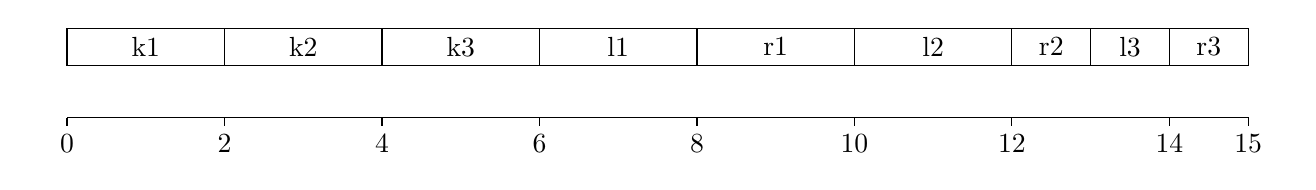
\begin{tikzpicture} [
    box/.style={draw,%
      outer sep=0,%
      align=center},
    bitc/.style={outer sep = 0,
      minimum width= 1cm,
      align = center}
    ]
    \node[box, minimum width=2cm] (h0) {k1};
    \foreach \i/\size/\name [remember=\i as \lastx (initially 0)] in {1/2cm/k2,2/2cm/k3,3/2cm/l1,4/2cm/r1,5/2cm/l2,6/1cm/r2,7/1cm/l3,8/1cm/r3} 
        \node[box, minimum width=\size, right= 0mm of h\lastx] (h\i) {\name};
    \node[bitc, below = 1cm of h0.west] (b0) {0};
    \draw (b0.north) -- +(0,.1);
    \foreach \i [remember=\i as \lasti (initially 0)] in {2,4,6,...,14} {%
      \node[bitc, right = 1cm of b\lasti] (b\i) {\i};
      \draw (b\i.north) -- +(0,.1) -- +(-2,.1);
    }
    \node[bitc, below = 1cm of h8.east] (b15) {15};
    \draw (b15.north) -- +(0,.1) -- + (-1,.1);
  \end{tikzpicture}
  \begin{description}
    \item[k?] Kind of operator \textit{?}.
    \item[l?] Left hand side operand index for operator \textit{?}.
    \item[r?] Right hand side operand index for operator \textit{?}.
  \end{description}
  \caption{Bit layout of a compressed tree in memory}
  \label{fig:comptree}
\end{figure}


\end{document}
